\subsection{Antennas}

In this sections, different antennas are placed in the TEM cell. Their electric and magnetic coupling is investigated through dipole moments. All antennas are fed with a power of 1\,W. Their material are made of a perfect electric conductor. Different positions and offsets are investigated and the results discussed. They are fed through a round wave port with a diameter of 0.46\,mm, and their wire has a diameter of 0.2\,mm and free-space permittivity. This results in a port impedance of 49.95\,$\Omega$. The TEM cell used has a width of $a=40$\,mm and a height of $b=24$\,mm, and its cells walls and septum consist of a perfect electric conductor, too. 


\todo[inline]{Describe how the use of normalization of ports influences results.}

\subsubsection{Monopole Antenna}

\begin{figure}[h]
	\centering
	\includegraphics[width=0.3\linewidth]{content/img/monopole_antenna}
	\caption{Geometry of monopole antenna inserted into the TEM cell.}
	\label{fig:monopoleantenna}
\end{figure}


\begin{figure}[htbp]
	\centering
	\begin{minipage}[t]{0.48\textwidth}
		\centering
		\includegraphics[width=1\linewidth]{content/img/dipole_moments_monopole.png}
		\caption{Dipole moments}
		\label{fig:dipole_moments_monopole}
	\end{minipage}
	\hfill
	\begin{minipage}[t]{0.5\textwidth}
		\centering
		\includegraphics[width=1\linewidth]{content/img/phase_shift_monopole}
		\caption{Phase shift}
		\label{fig:phaseshiftmonopole}
	\end{minipage}
\end{figure}
\todo{the length goes to 2mm}

The formula for dipole moments is used to calculate the dipole moments. The normalized electric field is constant over the frequency. But since the radiation resistance is expected to increase quadratically, we expect the dipole moments to rise linearly.

\autoref{fig:dipole_moments_monopole} shows the dipole moments of the monopole antenna. Note the linear relation of the electric dipole moment $m_\mathrm{e}$ to the frequency, which is not given in the center fed monopole and inverted-F antenna. The magnetic dipole moment equals zero, which is explainable by the very weak coupling of the magnetic fields. The length of the monopole antenna is 5\,mm.

The wave impedance in the near field region is very high in the low frequencies, but sharply drops off with frequency\todo{insert plot}. The relation is approximately given by \autoref{eqn:wave_impedance_monopole}, where $r$ describes the distance to the antenna.\todo{Source: \href{https://en.wikipedia.org/wiki/Near_and_far_field}{Wikipedia}. I couldn't find the source in the reference books. TODO} Generally, the near-field is electric, which is explaining by the capacitive behavior of the monopole antenna. The decrease of the wave impedance over the frequency also leads to better impedance matching, as the source impedance is set to 50\,$\Omega$. This leads to better power transfer, and more efficient radiation. \todo{Explain how much of the power transfer is due to the quadratic rise of the radiation resistance, and how much of it is due to better matching. As visible, in the current / voltage plots, the quadratic rise of the resistance influences the power transfer much more than the increased matching.} 

\begin{equation}
	\left|Z_\mathrm{w}\right| \approx 60\, \Omega \frac{c}{r\cdot f}
	\label{eqn:wave_impedance_monopole}
\end{equation}


\begin{figure}[h]
	\centering
	\includegraphics[width=1\linewidth]{content/img/monopole_surface_currents.png}
	\caption{Current surface density at 550\,MHz}
	\label{fig:monopole_surface_currents}
\end{figure}

\autoref{monopole_surface_current_offset} shows the induced surface currents on the septum, when giving the monopole antenna an offset of 7.5\,mm. The energy transfer decreases by 1\,dB.  

\begin{figure}[h]
	\centering
	\includegraphics[width=1\linewidth]{content/img/monopole_surface_current_offset.png}
	\caption{Current surface density at 550\,MHz with offset}
	\label{fig:monopole_surface_current_offset}
\end{figure}

\autoref{fig:monopolefeedcurrent} demonstrates the feed current over the frequency. Because the monopole antenna has a high impedance, the it rises linearly with the frequency. Meanwhile, the voltage falls quadratically with the frequency \todo{show plot and show mathematically}. This all fits together with the quadratic rise of the radiation resistance \todo{show mathematically?}. This evaluation has been done automatically through a script, integrating the magnetic field around the wire \todo{How big is the radius of the closed circle around the antenna. Sketch? What does the script look like}.


An equivalent circuit is derived in \autoref{fig:chucircuit}, which is known as Chu equivalent circuit for a short dipole \cite{Hansen_Collin_2013}. \todo{What is the purpose of this circuit here? Explain more. And should other chapters have circuits, too?}


\begin{figure}[h]
	\centering
	\includegraphics[width=0.3\linewidth]{content/img/chu_circuit}
	\caption{Chu equivalent circuit of short dipole}
	\label{fig:chucircuit}
\end{figure}


The distribution of the current along the monopole antenna is numerically derived by integrating the magnetic field strength in a closed loop around the antenna. \autoref{fig:currentdistributionmonopole} shows approximately a linear decrease of the current along the antenna, as assumed in \autoref{sec:dipoles}. \todo{Maybe increase resolution by adding more steps} A stronger decrease is visible near the feedpoint, which might occur due to the large displacement current density. An option to improve upon this simulation is increasing the feedpoint size, such that it has 50$\,\Omega$ impedance without needing port normalization.


\begin{figure}[htbp]
	\centering
	\begin{minipage}[t]{0.48\textwidth}
		\centering
		\includegraphics[width=1\linewidth]{content/img/current_distribution_monopole}
		\caption{Current distribution}
		\label{fig:currentdistributionmonopole}
	\end{minipage}
	\hfill
	\begin{minipage}[t]{0.48\textwidth}
		\centering
		\includegraphics[width=1\linewidth]{content/img/monopole_feed_current}
		\caption{Feed current}
		\label{fig:monopolefeedcurrent}
	\end{minipage}
\end{figure}



\FloatBarrier

\subsubsection{Loop antenna}\label{sec:loop_sim}

\begin{figure}[h]
	\centering
	\includegraphics[width=0.4\linewidth]{content/img/loop_antenna}
	\caption{Geometry of loop antenna inserted into the TEM cell. The return path leads into the conducting surface of the cell.}
	\label{fig:loopantenna}
\end{figure}


\todo[inline]{equivalent circuit in Balanis page 244}
\todo[inline]{inductance of square loop given in Balanis page245}

A loop antenna of dimensions in form of a square is constructed, with each size having a length of 1.6\,mm. This is preferable to a really round antenna, because the adaptive meshing models it much more accurate. \todo{Maybe describe this in the HFSS theory part? Modeling of round surfaces.} The antenna is oriented such that the highest amount of magnetic fields enters it.

\begin{figure}[h]
	\centering
	\includegraphics[width=0.7\linewidth]{content/img/loop_elec_energy}
	\caption{}
	\label{fig:loopelecenergy}
\end{figure}
\begin{figure}[h]
	\centering
	\includegraphics[width=0.7\linewidth]{content/img/loop_mag_energy}
	\caption{}
	\label{fig:loopmagenergy}
\end{figure}
\begin{figure}[h]
	\centering
	\includegraphics[width=0.7\linewidth]{content/img/loop_feed_current}
	\caption{}
	\label{fig:loopfeedcurrent}
\end{figure}
\begin{figure}[h]
	\centering
	\includegraphics[width=0.7\linewidth]{content/img/loop_feed_voltage}
	\caption{}
	\label{fig:loopfeedvoltage}
\end{figure}





\begin{figure}[h]
	\centering
	\includegraphics[width=1\linewidth]{content/img/dipole_moments_loop_antenna.png}
	\caption{Dipole moments of loop antenna}
	\label{fig:dipole_moments_loop_antenna}
\end{figure}

\autoref{fig:dipole_moments_loop_antenna} shows the dipole moments of the loop antenna over frequency. As expected, the magnetic dipole moment $_\mathrm{m}$ contributed the largest amount to the antenna coupling. A small amount of electric dipole moment is also present, which naturally occurs due to the current wire aligned with the TEM electric fields. The electric dipole moment $m_\mathrm{e}$ increases non-linearly with frequency. \todo{why?}

\begin{figure}[h]
	\centering
	\includegraphics[width=1\linewidth]{content/img/current_loop_surface_current.png}
	\caption{Surface current density at 550\,MHz}
	\label{fig:current_loop_surface_current}
\end{figure}




Note that the surface current density in \autoref{fig:current_loop_surface_current} is much more concentrated in the center. In the case of the monopole antenna, the current density distributed almost equally around the septum. In the case of the loop antenna, the current below the antenna seems to be cut off by the rotational eddy currents next to them. \todo{Find reasons for the eddy current to exist. Maybe there is a nice formula that describes this by maxwell?} Furthermore, the phase shift between the currents at the output ports is 180°, leading to the perceived phase shift of magnetic dipole moments.

\autoref{fig:current_loop_surface_current_offset} demonstrates the surface current density when shifting the loop antenna 7.5\,cm (quarter of the septum width) in y-direction. The coupling and transferred energy remains roughly the same.

\begin{figure}[h]
	\centering
	\includegraphics[width=1\linewidth]{content/img/current_loop_surface_current_offset.png}
	\caption{Surface current density at 550\,MHz with offset}
	\label{fig:current_loop_surface_current_offset}
\end{figure}

\autoref{fig:current_loop_surface_current_rotated} shows the surface current density when rotating the antenna by 90°. Only a negligible amount reaches the output ports, leading to no coupling.  

\begin{figure}[h]
	\centering
	\includegraphics[width=1\linewidth]{content/img/current_loop_surface_current_rotated.png}
	\caption{Surface current density at 550\,MHz with rotated antenna}
	\label{fig:current_loop_surface_current_rotated}
\end{figure}

\autoref{fig:current_loop_surface_current_offset_rotated} shows the current distribution of the current loop antenna, when it is rotated and contains an offset. Again, the eddy currents dominate. However, some of those currents propagate towards the output ports, increasing the energy transfer minimally (0.5\,dB). Additionally, the energy transferred is in phase, which makes it indistinguishable from an electric dipole.

\begin{figure}[h]
	\centering
	\includegraphics[width=1\linewidth]{content/img/current_loop_surface_current_offset_rotated.png}
	\caption{Surface current density at 550\,MHz with offset and rotated antenna}
	\label{fig:current_loop_surface_current_offset_rotated}
\end{figure}

\todo{annotate maximum and minimum current densities}



\autoref{fig:currentloopchargedistribution} shows the charge density distribution in the current loop antenna. Charges collect, among other locations, at the bottom wire. This leads to electric coupling with the septum. 

\begin{figure}[htbp]
	\centering
	\begin{minipage}[b]{0.45\textwidth}
		\centering
		\includegraphics[width=0.5\linewidth]{content/img/current_loop_charge_distribution}
		\caption{Charge density distribution in current loop antenna}
		\label{fig:currentloopchargedistribution}
	\end{minipage}
	\hfill
	\begin{minipage}[b]{0.45\textwidth}
		\centering
		\includegraphics[width=0.5\linewidth]{content/img/current_loop_current_distribution}
		\caption{Current density distribution in current loop antenna}
		\label{fig:currentloopcurrentdistribution}
	\end{minipage}
\end{figure}


The current and voltage drops along the wire are not constant. From the feedpoint to the first corner, there is a much larger voltage drop and current, than from the second corner to the ground plane. Consequently, the power consumed by the first part is much higher than by the latter \todo{Insert power consumption plots of each antenna section}. Additionally, this difference in power consumption increases slightly over frequency. 

The electric current reduces over the wire because of the displacement current to the septum and the ground plane. As visible in the charge density plot in \autoref{fig:currentloopcurrentdistribution} and the electric field plot in \autoref{fig:currentloopnearefield}, much of the displacement current occurs near the feedpoint and at the wire parallel to the septum. Consequently, this is where the current drops by the most amount. \todo{Insert current distribution plots}



\begin{figure}[htbp]
	\centering
	\begin{minipage}[b]{0.45\textwidth}
		\centering
		\includegraphics[width=0.7\linewidth]{content/img/current_loop_near_e_field}
		\caption{Electric near field in current loop antenna}
		\label{fig:currentloopnearefield}
	\end{minipage}
	\hfill
	\begin{minipage}[b]{0.45\textwidth}
		\centering
		\includegraphics[width=0.7\linewidth]{content/img/current_loop_near_h_field}
		\caption{Magnetic near field in current loop antenna}
		\label{fig:currentloopnearhfield}
	\end{minipage}
\end{figure}


\todo{H-field from other perspective?}

\begin{figure}[htbp]
	\centering
	\begin{minipage}[b]{0.45\textwidth}
		\centering
		\includegraphics[width=1\linewidth]{content/img/current_loop_voltage_drop}
		\caption{Voltage drop at feed point of current loop antenna}
		\label{fig:currentloopvoltagedrop}
	\end{minipage}
	\hfill
	\begin{minipage}[b]{0.45\textwidth}
		\centering
		\includegraphics[width=1\linewidth]{content/img/current_loop_feed_current}
		\caption{Current consumption at feed point of current loop antenna}
		\label{fig:currentloopfeedcurrent}
	\end{minipage}
\end{figure}

\autoref{fig:currentloopfeedcurrent} and \autoref{fig:currentloopvoltagedrop} show the current and voltage consumption of the antenna. The phase shift equals $\phi\approx89.80\circ$, which hints to a strong inductive behavior. The inductance is determined to be $L\approx2.15\,\mathrm{nH}$. The capacitance is very low, but does lead so some displacement current. The frequency behavior of the voltage and current interchange if the antenna is strongly capacitive, as it the case in a monopole antenna.

A theoretical approach to approximate the inductance of a current loop in free-space is \cite[p. 245]{Balanis_1997}

\begin{equation}
	L_A = \frac{2\mu_0 a}{\pi} \left[ \ln\!\left(\frac{a}{b}\right) - 0.774 \right],
\end{equation}

which yields $L=2.56\,\mathrm{nH}$. However, this does not consider the coupling effects of the TEM cell.


Next, the electric and magnetic near field is investigated. The wave impedance $Z=E/H$ shown in \autoref{fig:waveimpedanceloop} in the center of the loop rises linearly over frequency. At low frequencies, the wave impedance is very low, which confirms the inductive behavior of the antenna. However, as the frequency increases, so does the voltage drop. This may be analogous to a inductor in an electrical circuit, across which the voltage drop also increases with frequency $U = \mathrm{i}L\omega I$. 

\begin{figure}[h]
	\centering
	\includegraphics[width=0.5\linewidth]{content/img/wave_impedance_loop}
	\caption{Wave impedance in the center of the loop}
	\label{fig:waveimpedanceloop}
\end{figure}

\autoref{eqn:a_b_moments_simp} relates the dipole moments to the output power. The influence of the dipole moments is determined by the electric field at the electric dipole moment and the magnetic field at the magnetic dipole moment. In this formula, the electric and magnetic field are simply related through the free-space wave impedance. However, as visible in \autoref{fig:waveimpedanceloop}, the wave impedance at the location of the dipole moments (i.e. at the antenna) is much lower. Additionally, it rises linearly with the frequency. This influence of the antenna itself on the fields around the dipoles could explain the non-linear relation of the dipole moments to the frequency.



\autoref{fig:currentlooppowerconsumption} shows the power consumption of the antenna, which is influenced by two factors. The radiation resistance rises quadratically with the frequency. At the same time, the impedance increases, leading to higher matching and therefore to a higher power transfer. This is contrary to the monopole antenna, where the impedance is decreases over the frequency, again leading to better impedance matching, because the impedance was high to begin with. The source impedance is 50\,$\Omega$.

\begin{figure}[h]
	\centering
	\includegraphics[width=0.5\linewidth]{content/img/current_loop_power_consumption}
	\caption{Power consumption of the current loop antenna}
	\label{fig:currentlooppowerconsumption}
\end{figure}

\autoref{fig:deleteafter} shows the total power maintained in the system, meaning $S_{11}^2+S_{12}^2+S_{13}^2$. It does not add up to one, meaning that some energy is lost due to finite conductivity of the septum and antenna. This energy dispersion increases with frequency, most likely due to a decrease of the conductivity due to high-frequency effects like the Skin-effect. Consequently, the power consumption in \autoref{fig:currentlooppowerconsumption} shows a square root relation to the frequency, because the power dispersion is so high. When changing the material of the antenna and septum to a perfect electric conductor, the total power in a system remains one (no power is dispersed) and the power consumption over frequency of the antenna shows a quadratic relation to the frequency, due to the quadratic increase of the radiation resistance.

\begin{figure}[h]
	\centering
	\includegraphics[width=0.7\linewidth]{content/img/delete_after}
	\caption{Total power distribution in the system}
	\label{fig:deleteafter}
\end{figure}

\begin{figure}[h]
	\centering
	\includegraphics[width=0.7\linewidth]{content/img/curr_loop_opower}
	\caption{Power and electric field at output port}
	\label{fig:currloopopower}
\end{figure}




The Skin-effect reduces the area in which the current flows, therefore increasing resistance. This appears due to the reduction of the depth, in which the electromagnetic waves enter. It is also called Skin depth and mathematically described by \autoref{eqn:skin_depth}. It depends on the imaginary part of the wave number $\kappa$, which is described in \autoref{eqn:kappa}. For high conducting materials $\left(\sigma >> \epsilon\omega\right)$, the dependency of the skin depth $d$ on the frequency can be described therefore as $d \propto 1/\sqrt{\omega}$. Since the power dispersion is linearly proportional to the area of the conductor and therefore Skin-depth, it shows the same dependency on the frequency $P_\mathrm{disp}\propto 1/\sqrt{\omega}$ \cite{Griffiths_2024}.  
\todo{Own little chapter for skin effect? Loop antennas are known for higher conductor losses than radiation Balanis page 231}

\begin{subequations}
	\begin{equation}
		\kappa = \omega \sqrt{\frac{\epsilon \mu}{2}}\left[\sqrt{ 1+\left(\frac{\sigma}{\epsilon\omega}\right) ^2 } -1\right]^{1/2}
		\label{eqn:kappa}
	\end{equation}
	\begin{equation}
		d = 1/\kappa
		\label{eqn:skin_depth}
	\end{equation}
\end{subequations}

At 1\,GHz, the dispersed power already equals to 0.46\,\%, which is much higher than the power transfer of the antenna to one waveport of 1.26e-5 at that frequency. Because this dispersed power is proportional to the square-root of the frequency $P_\mathrm{disp}\propto 1/\sqrt{\omega}$, the overall transferred power to the antenna shows the same characteristic. However, the power transfer to the waveports has a quadratic dependency on the frequency. %This, in turn, also leads to the unusual relation of the electric dipole moment to the frequency. 
\todo{explain better.}

This dispersed power may be ignored in the simulations by changing the antenna's material (main source of power dissipation) and the septum from copper to a perfect electric conductor. The overall power in the system then remains at a constant one over the whole frequency range. Additionally, the transferred power to the antenna now has a quadratic relationship with the frequency, indicating increased radiation efficiency, previously described by \autoref{eqn:elec_rad_res}. 
\todo{Show plots?}


The current-loop antenna contains two electric dipoles, shifted in phase by 180°. They therefore oppose each other in the power transfer to the waveports. However, as visible in the electric near field plot in \autoref{fig:currentloopvoltagedrop}, the electric dipole moment from node A to the feedpoint is much larger than the one from node B to ground. The reason can be demonstrated by representing the antenna with its nodes in \autoref{fig:current_loop_ua_ub}. The partial inductances in this schematic are much larger than the capacitances. This leads to a large voltage drop between node A and B, and therefore a weaker electric dipole moment at node B.

Additionally, this voltage difference $V_\mathrm{A}-V_\mathrm{B}$ rises linearly over the frequency, due to the linearly increasing impedance of the inductance $\mathrm{i}\omega L$. This means, that the over electric dipole moment a quadratic relationship to the frequency has.
\todo{Magnetic moment equivalent antenna. Explain with current and H-field, too}

\todo{Prove square frequency dependency}

Further, \autoref{fig:loopwaveimp} shows the wave impedance of the near-fields at the loop antenna. The \autoref{eqn:a_b_moments_simp} shows, that the influence of the dipoles depends on the electric and magnetic fields at the dipoles position. The electric and magnetic fields are related through the wave impedance $Z = E/H$. If the wave impedance rises linearly over frequency, the electric field increases over the magnetic fields, giving more influence to the electric dipole moments. As previously discussed, there are two electric dipole moments in this antenna, benefiting from that. \todo{Monopole antenna: Also change in wave impedance, but there is not really a magnetic dipole moment} 

\begin{figure}[h] 
	\centering
	\includegraphics[width=0.7\linewidth]{content/img/loop_wave_imp}
	\caption{Wave impedance in near field of loop antenna over frequency}
	\label{fig:loopwaveimp}
\end{figure}

The wave impedance $Z_\mathrm{w}$ in the near field of the electrically small loop antenna is approximated by \autoref{eqn:wave_impedance_loop}. It confirms the linear relationship of the near-field wave impedance to the frequency. \todo{Source: \href{https://en.wikipedia.org/wiki/Near_and_far_field}{Wikipedia}. I couldn't find the source in the reference books. TODO}


\begin{equation}
	\left|Z_\mathrm{w}\right|\approx 2 \pi^2 \cdot 240\,\Omega \cdot\frac{r\cdot f}{c}
	\label{eqn:wave_impedance_loop}
\end{equation}



\FloatBarrier

\subsubsection{Inverted F-antenna}\label{sec:ifa_sim}

The inverted F-antenna (IFA) is modeled in Ansys HFSS as shown in \autoref{fig:ifa}. It is positioned at the center of the TEM cell, mounted at the top surface. The 5\,mm long wire points towards waveport 2. The excitation is a modal wave port. With a maximum dimension of 5\,mm, the antenna is electrically small for a frequency of up to 6\,GHz, at which it will be a tenth of the wavelength. In this simulation, the antenna is investigated for the frequency of 100\,MHz to 1\,GHz. The TEM cell has a width of 40\,mm and a height of 24\,mm and an impedance of $\sim50\,\Omega$. The goal is to find equivalent dipole moments of the antenna. 


\begin{figure}[h]
	\centering
	\includegraphics[width=0.75\linewidth]{content/img/inverted_f_antenna.png}
	\caption{Inverted F-antenna used in the simulation}
	\label{fig:ifa}
\end{figure}

The coupling between the antenna and the two ports of the TEM cell are described by S-parameters, specifically the forward transmission coefficients $S_{\mathrm{A1}}$ and $S_{\mathrm{A2}}$. \autoref{fig:antenna_waveport1_sparams} shows the magnitude of this coefficient, which is the same for the antenna to both ports ($|S_{\mathrm{A1}}|=|S_{\mathrm{A2}}|$). 


\begin{figure}[h]
	\centering
	\includegraphics[width=1\linewidth]{content/img/antenna_waveport1_sparams.png}
	\caption{S-parameter describing coupling of antenna to waveport 1}
	\label{fig:antenna_waveport1_sparams}
\end{figure}

\begin{equation}
	P_{\mathrm{Antenna}}=\frac{P_{\mathrm{Out1}}}{10^{|S_{\mathrm{A1}}|/10}}=\frac{P_{\mathrm{Out2}}}{10^{|S_{\mathrm{A2}}|/10}}
	\label{eqn:power_antenna}
\end{equation}


\autoref{eqn:power_antenna} describes the relation between the input power at the antenna and the measured output power of the TEM cell. It is defined by the magnitude of the forward transmission coefficients.

\begin{equation}
	\iint_A \mathbf{e_0} \times \mathbf{h_0} \cdot\mathrm{d}\mathbf{A} = 1
	\label{eqn:normalization of fields}
\end{equation}

\autoref{eqn:normalization of fields} shows that the electric field $\mathbf{e_0}$ and magnetic field $\mathbf{h_0}$ are normalized to $1\,\sqrt{\mathrm{W}}$. The surface area $A$, over which the fields are integrated, is that of the output ports of the TEM cell. The field can be linearly scaled by the complex coefficients $a$ and $b$, which has been described in \autoref{eqn:modal_superposition1} and \autoref{eqn:modal_superposition2}. Only one pair of such coefficients is needed, since only the TEM mode is considered.

The coefficients $a$ and $b$ have the unit $\sqrt{\mathrm{W}}$. The fields $\mathbf{e_0}$ and $\mathbf{h_0}$ are not known over the whole area. However, the electric field $\mathbf{e_0}$ has only to be known at one specific point in order to determine the equivalent dipole moments, as will be shown here. The normalization condition therefore leads to an output power equal to $|a|^2/2$ or $|b|^2/2$, respectively, which was also found in \cite{4091811}.

\begin{subequations}
	\begin{equation}
		P_{\mathrm{out1}}=\iint_A \langle \mathbf{S} \rangle \cdot \mathrm{d}\mathbf{A}= \iint_A \frac{1}{2} \, \Re \{ \left(a\cdot \mathbf{e_0}\right) \times \left(a\cdot \mathbf{h_0}^*\right) \}\cdot \mathrm{d}\mathbf{A} = \frac{|a|^2}{2}
		\label{eqn:power_of_poynting1}
	\end{equation}
	\begin{equation}
		P_{\mathrm{out2}}=\iint_A \langle \mathbf{S} \rangle \cdot \mathrm{d}\mathbf{A}= \iint_A \frac{1}{2} \, \Re \{ \left(b\cdot \mathbf{e_0}\right) \times \left(b\cdot \mathbf{h_0}\right)^* \}\cdot \mathrm{d}\mathbf{A} = \frac{|b|^2}{2}
		\label{eqn:power_of_poynting2}
	\end{equation}
\end{subequations}



The phase shifts of $S_{\mathrm{A1}}$ and $S_{\mathrm{A2}}$ differ, which is shown in \autoref{fig:phase_shift_waveports_ifa}. The difference of these phase shifts influences the quantity of magnetic dipole moment and electric dipole moments. A large phase shift indicated a large magnetic dipole moments compared to the electric dipole moment, and vice versa. The large difference in phase shifts in \autoref{fig:phase_shift_waveports_ifa} lets one expect the first case. However, the phase shift does not influence the overall output power. It is incorporated into the coefficients $a$ and $b$, by multiplying the term $e^{\mathrm{i}\varphi_{a}}$ or $e^{\mathrm{i}\varphi_{b}}$ to their magnitude. The phase shift of each port is then implemented by $\varphi_{a}$ at the port of the coefficient $a$, and by $\varphi_{b}$ at the port of the coefficient $b$. 

The Poynting vector is periodic from $-\pi/2$ to $\pi/2$, hence any phase difference above that value must be corrected by adding $\pi$ to it. 

\begin{figure}[h]
	\centering
	\includegraphics[width=1\linewidth]{content/img/Phase Shift Waveports.png}
	\caption{Phase of S-parameters from antenna to waveport 1 and 2}
	\label{fig:phase_shift_waveports_ifa}
\end{figure}

The output power of each port is then derived through \autoref{eqn:power_of_poynting1} and \autoref{eqn:power_of_poynting2}. So if $|a|=|b|=1$, then the electric field $\mathbf{e_0}$ may be measured, when the output power at one port is $\frac{1}{2}\,\mathrm{W}$. Because it is assumed that the TEM cell contains only waves in the TEM mode, the normalization of the electric and magnetic fields can be used to simplify the calculations.

\begin{equation}
	\mathbf{e_0}\times\mathbf{h_0}=\Re\{\mathbf{e_0}\times\mathbf{h_0}^*\} \quad\text{for TEM mode}
	\label{eqn:equivalent_tem}
\end{equation}

\todo{Problem with large TEM cell: Formula does not work for large frequencies. The field distributes around the port. Describe this. Error grows with frequency}

By using \autoref{eqn:mag_dipole_moment_tem} and \autoref{eqn:dipole_tem_waves}, the equivalent dipole moments are derived. Because of Lorentz reciprocity theorem, only fields aligned with the dipole moments get to the output ports. Since only the TEM mode propagates, only the electric dipole moment in z-direction and the magnetic dipole moment in y-direction influence the fields. If higher order modes can propagate, the other dipole moments become relevant, too.
\todo{Einheitliches Koordinatensystem definieren}



\begin{equation}
	m_{\mathrm{e}}=\frac{a+b}{e_{0,z}}
	\label{eqn:ifa_me}
\end{equation}

\begin{equation}
	m_{\mathrm{m}}=\mathrm{i}\frac{a-b}{k_0  e_{0,z}}
	\label{eqn:ifa_mm}
\end{equation}

By adding or subtracting the coefficients $a$ and $b$, the dipole moments are expressed into the handy \autoref{eqn:ifa_me} and \autoref{eqn:ifa_mm}. There, $k_0=\frac{2\pi}{\lambda}$ is the free space wave number and $e_{0,z}$ is the normed electric field in z-direction at middle height between septum and the upper wall of the TEM cell. However, the height of the measurement point is not important, as the electric field is uniformly distributed along the z-axis. Additionally, the x- and y-components of the electric field $\mathbf{e_{0}}$ are zero, which leads to these equations. The dipole moments $m_{\mathrm{e}}$ and $m_{\mathrm{m}}$ are defined to be in the center of the TEM cell, at middle height. If they are shifted in any direction, their approximation would not hold true anymore.

\begin{figure}[h]
	\centering
	\includegraphics[width=1\linewidth]{content/img/sketch_dipoles_tem_cell.png}
	\caption{Dipole moments and measurement point of $e_{0,z}$ in TEM cell}
	\label{fig:sketch_dipoles_tem_cell}
\end{figure}

\autoref{fig:sketch_dipoles_tem_cell} shows the measurement point of $e_\mathrm{0,z}$. This wouldn't work if the magnetic and electric dipole wasn't defined to be exactly at a height of $b/4$, at dead center. The Lorentz Reciprocity theorem used to derive the formulas take the cross product of the electric field traveling to one output port with the magnetic field caused by the dipole, minus the magnetic field traveling to the same output port minus the electric field caused by the dipole. Since the dipoles are in dead center, the electric field caused by the dipole does only have a z-component, and the magnetic field caused by the dipole only a y-component. If this was not the case, the other components would have to be taken into account of the fields at the test point. They would already have disappeared at the output ports due to the long travel, and the Lorentz Reciprocity theorem becomes more cumbersome to use. By placing the dipoles in dead center, it is possible to measure the electric field at the output port and normalize it to $\frac{1}{2}\,\mathrm{W}$.

\todo{Write clearer. And put into theoretical part.}

Using \autoref{eqn:magn_current_curr_loop} the magnetic dipole moment can be expressed as a magnetic current. The resulting $m_{m,mag}$ is shown in \autoref{eqn:m_mymag_ifa}. The phase shift between the magnetic and electric dipole moments $m_{\mathrm{ez}}$ and $m_{\mathrm{my,mag}}$ is always $\frac{\pi}{2}$, which generates the desired TEM wave pattern.

\begin{equation}
	m_{\mathrm{m,mag}}=\mathrm{i}m_{\mathrm{m}}\omega\mu_0
	\label{eqn:m_mymag_ifa}
\end{equation}

The antenna may then be replaced with those two dipole excitations in the center of the upper half of the TEM cell. The magnitude and phase of the fields, as well as the output powers, should remain the same as in the case with the antenna. The phase shift may be determined by measuring the phase shifts of the electric fields at both output ports. When applying this described method in a measurement with a real TEM cell, the phase shift may be found by adding and subtracting the output powers of both ports, as is shown in \cite{Sreenivasiah_Chang_Ma_1981}.

\begin{figure}[h]
	\centering
	\includegraphics[width=1\linewidth]{content/img/dipole_moments_over_freq_ifa.png}
	\caption{Dipole moments over frequency}
	\label{fig:dipole_moments_over_freq_ifa}
\end{figure}


\todo{Is this CFM or IFA simulation?}




\autoref{fig:dipole_moments_over_freq_ifa} shows the dipole moments over frequency. The electric dipole moment $m_e$ has been normalized to the free-space wave impedance of $377\,\Omega$ to make the dipole moments comparable. This is possible because the dipole moments are interchangeable through the wave impedance \cite[p. 414]{Jackson}. The antenna input power has been set to 142588.47\,W, because this leads to an output power of 1\,W at a frequency of 1\,GHz. The magnetic dipole moment is much larger than the electric dipole moment, because the current loop of the antenna is aligned with the TEM cell's magnetic fields, but the line current is not with the TEM electric fields. The magnetic dipole moments rises linearly with the frequency, which is equal to a quadratic increase of power. Only the TEM modes has been considered in the simulation, as other modes disturb the calculations. 

The electric field $\mathbf{e_0}$ is approximated with \autoref{eqn:ifa_e_field_approx} for the purpose of interpolation over frequencies and analytical analysis. The constant $u$ is a scaling factor, which must be adjusted to fit the real electric field values. In this case, this constant equals $u=820.34$. The left-hand side term $|a|\cdot e_{0,z}$ is the overall electric field at the measurement point according to \autoref{eqn:modal_superposition1}. \autoref{fig:output_power_e_fields_over_freq_ifa} shows the resulting plot. 

\begin{equation}
	|a|\cdot e_{0,z}=\sqrt{2P_\mathrm{Out}}\cdot e_{0,z}=u\sqrt{P_\mathrm{Out}}\,\mathrm{\frac{V}{m\cdot\sqrt{W}}}
	\label{eqn:ifa_e_field_approx}
\end{equation}

\begin{figure}[h]
	\centering
	\includegraphics[width=1\linewidth]{content/img/output_power_e_fields_over_freq_ifa.png}
	\caption{Output power and electric field over frequency}
	\label{fig:output_power_e_fields_over_freq_ifa}
\end{figure}

The electric field can also be approximated by \autoref{eqn:e_field_at_one_point}, where $b/2=12\,\mathrm{mm}$ is half the height and $Z_\mathrm{W}\approx50\,\Omega$ is the impedance of the TEM cell. This works for TEM cells with thin septum. The constant $u$ can be adjusted to fit this equation. The term $\sqrt{2}$ is needed to convert the effective value of the electric field into its magnitude.

\begin{equation}
	|a|\cdot e_{\mathrm{0,z}}=\frac{\sqrt{2\cdot P_\mathrm{Out}\cdot Z_\mathrm{W}}}{b/2}
	\label{eqn:e_field_at_one_point}
\end{equation}

\todo{Repeat for different orientations? Change variable name: TEM cell height.}

The magnetic coupling with the septum happens due to the alignment of the current loop with the magnetic field of the dominant TEM mode. The antenna is now rotated by 90° around the z-axis, such that the magnetic current loop stands perpendicular to the magnetic TEM fields. \autoref{fig:phase_shift_90_ifa} demonstrates the phase of the S-parameters, describing the coupling of antenna to waveport 1 and 2. Since the magnetic dipole moment is responsible for a phase between the ports, \autoref{fig:phase_shift_90_ifa} strongly hints to an absence of it.

\begin{figure}[h]
	\centering
	\includegraphics[width=1\linewidth]{content/img/phase_shift_90_ifa.png}
	\caption{Phase of S-parameters from rotated antenna to waveport 1 and 2}
	\label{fig:phase_shift_90_ifa}
\end{figure}

\autoref{dipole_moments_ifa_90} shows that the electric dipole moment $m_\mathrm{e}$ has stayed the same, while the magnetic dipole moment became zero. Consequently, the overall power transfer between the antenna and the waveports is also much lower. 

\todo{The same procedure was repeated with different dipole moments positions, for which \autoref{eqn:e0z_mse} worked. Maybe do a general equation for the normalized e-field?}

\begin{figure}[h]
	\centering
	\includegraphics[width=1\linewidth]{content/img/dipole_moments_ifa_90.png}
	\caption{Dipole moments of rotated antenna}
	\label{fig:dipole_moments_ifa_90}
\end{figure}


\FloatBarrier
\subsubsection{Center Fed Monopole Antenna}

The center fed monopole antenna is shown in \autoref{fig:center_fed_monopole}. The conducting plane in \autoref{fig:center_fed_monopole} is on the top side of the TEM cell, thus the image is rotated counter-clockwise by 90 degrees. The electric wire with the length of 5 mm points towards the septum. The 1.1 x 1.6 mm loop is again aligned with the magnetic field lines of the TEM mode. The antenna is fed with a power of $P_\mathrm{Antenna}=127770.39\,\mathrm{W}$, which once more leads to an output power of $P_\mathrm{Out}=1\,\mathrm{W}$ at 1\,GHz at both output ports. 

\begin{figure}[h]
	\centering
	\includegraphics[width=0.75\linewidth]{content/img/center_fed_monopole.png}
	\caption{Center fed monopole antenna used in simulation}
	\label{fig:center_fed_monopole}
\end{figure}

The magnitude of $|S_\mathrm{A1}|=|S_\mathrm{A2}|$ in \autoref{fig:forward_coeff_cfm} shows stronger coupling. As will be seen below, this is because of an increased electric dipole moment, while the magnetic dipole moment remained the same. Therefore, the center fed monopole antenna couples well electrically with the TEM cell.

\begin{figure}[h]
	\centering
	\includegraphics[width=1\linewidth]{content/img/forward_coeff_cfm.png}
	\caption{S-parameter describing coupling of antenna to waveport 1}
	\label{fig:forward_coeff_cfm}
\end{figure}

%The phase shift in \autoref{fig:phase_shift_cfm} is smaller than in the simulation with the inverted F antenna. This hints to a more influential electric dipole moment than before. This is because of the term $a+b$... When using superposition of each dipole moment...
%
%\begin{subequations}
%	\begin{equation}
%		c_1 = \sqrt{a^2+b^2+2ab\cos{\left[ (\varphi_a + \varphi_b) / 2 \right]}}
%	\end{equation}
%	\begin{equation}
%		c_2 = \sqrt{a^2+b^2-2ab\sin{\left[ (\varphi_a - \varphi_b) / 2 \right]}}
%	\end{equation}
%	\begin{equation}
%		c_1^2+c_2^2= a^2+b^2
%	\end{equation}
%\end{subequations}
%\todo{not done yet, make it correct}







\begin{figure}[htbp]
	\centering
	\begin{minipage}[t]{0.48\textwidth}
		\centering
		\includegraphics[width=1\linewidth]{content/img/phase_shift_cfm.png}
		\caption{Phase shift}
		\label{fig:phase_shift_cfm}
	\end{minipage}
	\hfill
	\begin{minipage}[t]{0.48\textwidth}
		\centering
		\includegraphics[width=1\linewidth]{content/img/dipole_moment_cfm.png}
		\caption{Dipole moments}
		\label{fig:dipole_moment_cfm}
	\end{minipage}
\end{figure}


\autoref{fig:dipole_moment_cfm} shows that the magnetic dipole moments of the inverted F and center fed monopole antennas are equal. This is due to the same size of the current loops. However, the electric dipole moments increased for the center fed monopole antenna. The alignment of the line current with the TEM cell's electric field causes this. (antenna power = 126549.7191667088\,W)



The output power has been scaled as in the simulation before. This leads to the same electric field magnitude. Therefore, the electric field and output power over frequency plot are the same as in the case for the inverted F antenna, visible in \autoref{fig:output_power_e_fields_over_freq_ifa}.


When rotating this antenna by 79°, the electric and magnetic dipole moment influence the output power by roughly the same amount, as visible in \autoref{fig:79cfm}. This makes itself manifest by a phase shift of around 45°  between the output powers of the waveports. Interestingly, both the electric and the magnetic dipole moment demonstrate a non-linear behavior. \todo{Why does the magnetic moment sink?}

\todo{CFM at 90° rotation still demonstrates magnetic dipole moment, opposed to current loop. Does this scale with antenna height, i.e. electric dipole moment?}

\FloatBarrier



\subsubsection{Serial Loop Antenna}

This section will discuss the antenna displayed in \autoref{fig:serialloopantenna}. The idea of that antenna is to create two magnetic dipole moments, which are in phase. As the frequency increases, the displacement current between the loops becomes larger, thus reducing the current through and weakening the second loop. The dipole moments in \autoref{fig:serialloopantennadipolemoments} demonstrate a non-linear behavior of the magnetic dipole moment (only very weakly recognizable, but with a geometry sweep this becomes clearer \todo{Find a geometry where this effect is much stronger}). Also, it would be interesting to measure the wave impedances in both loops over the frequency. Also, find the current distributions, add current plots and electric fields, charge distributions.  

\begin{figure}[h]
	\centering
	\includegraphics[width=0.3\linewidth]{content/img/serial_loop_antenna}
	\caption{Serial loop antenna}
	\label{fig:serialloopantenna}
\end{figure}
\begin{figure}[h]
	\centering
	\includegraphics[width=1\linewidth]{content/img/serial_loop_antenna_dipole_moments}
	\caption{Dipole moments }
	\label{fig:serialloopantennadipolemoments}
\end{figure}

\FloatBarrier

\subsubsection{Offset of source antennas and eddy currents}

\todo{Relate the offset to the normalized E field distribution. For Example, the vertical part of the current loop antenna does not influence the TEM cell coupling without offset, which can be shown with the normalized E field distribution.}

\todo{Can the normalized h-field distribution be related to the E field by multiplying it with the free-space wave impedance? How does a 90° rotated current loop antenna couple with offset? There should be some coupling due to the existence of normalized h-fields there}

\colorbox{red}{This section is probably wrong.}

Next, the CFM is rotated by an angle. This angle is swept from 0° to 90°, iteratively increased by 1° [deg]. At 90° the magnetic dipole moment is at a minimum, while it is the largest at 0°. The idea is now to find a balance between the electric and magnetic dipole moment, such that the antenna operates in a way of resonance. In this operation, the S11 parameter shall be the lowest, even though the coupling of the magnetic field only becomes weaker with increasing angle \todo{Is it possible to proof this by mathematics?}. The reason for this approach by increasing angle is that it is otherwise very hard to achieve such a balance between the dipole moments by purely scaling the antenna. The electric dipole moment is very weak, and when increasing the antenna height (thus only the electric dipole moment), it soon becomes very large and even touches the septum. Rotating the angle instead becomes a very efficient alkternative. This has been determined just by looking at the phase shifts from the antenna to the waveports: If electric and magnetic dipole moments are roughly equally influential, then the phase shift between the ports shall be 90°\todo{Show mathematically?}. Very important for these simulation is the renormalization of the waveports \todo{Describe this in HFSS section, under excitations}. This enables the port exciting the antenna to have an impedance of 50 Ohm, independent of size. This will make a geometry sweep of the antenna able, without influencing the impedance of the port exciting the antenna (Imagine a coax cable attached to the antenna. It is hinted by the round waveport in the model. When it gets shifted around, its wave impedance changes, and so does the reflection, and the results are distorted) 




\FloatBarrier

\autoref{fig:cfm_rotation_sweep} it is visible, that the lowest S11 (least reflections) is achieved at a rotation angle of 72°. \todo{Why, how do the dipole moments look like there? Anf is this just a numerical error?}

\begin{figure}[h]
	\centering
	\includegraphics[width=1\linewidth]{content/img/cfm_rotation_sweep.png}
	\caption{CFM S11 sweep with rotation angle stepping}
	\label{fig:cfm_rotation_sweep}
\end{figure}


Eddy currents occur on the septum. They increase with frequency. When they get too large, the next-order mode starts propagating. Offsetting the antenna / dipole moment in y-direction reduces the amount of influence of the eddy current on the power carrying current in the septum. 

\todo{How does offset influence the eddy currents and the result?}


When implementing an offset in the center fed monopole antenna, the coupling between the waveports and the antenna changes. The change is visible in \autoref{fig:DELETE_AFTER}, although the magnitude of the coupling to both ports is the same.

\todo{Better investigation of offset: Show coupling and eddy currents}

\begin{figure}[h]
	\centering
	\includegraphics[width=1\linewidth]{content/img/DELETE_AFTER.png}
	\caption{Center fed monopole antenna coupling dependence on offset (Delete after)}
	\label{fig:DELETE_AFTER}
\end{figure}

